\section{Background and Related Work}
Low-level systems software depends on correct algorithms but also on
how data is represented in memory. Choices about field order, alignment, and
bit layout can affect performance, portability, and correctness. This chapter
surveys research and industrial work that informs Cedar's design. It begins
with an overview of the problem space, followed by a 
discussion.of C's memory model and layout hazards.
The chapter then examines verified compilers and formal memory 
models, declarative and industrial data-layout
languages,
and runtime analysis tools for detecting memory errors.
The final section synthesizes these threads and
identifies the gap that motivates Cedar's contribution.

\subsection{Overview} \label{5-background}
Precise control over data representation is a defining features of systems
programming. Languages such as C give programmers direct access to memory
through pointers and explicit layout constructs, enabling high-performance
and hardware-proximate code~\autocite{memory_bottleneck, C_embedded_programming}.
At the same time, this flexibility introduces persistent risks: implicit
padding, inconsistent alignment across architectures, and aliasing behaviors
that are only partly defined by the C
standard~\autocite{whatyouc, strict_aliasing}. Even when program logic is
sound, representation errors can lead to subtle faults, security
vulnerabilities, or degraded cache
performance~\autocite{memory_errors_stridharan, C_errors_study, adt_layout_faria}.

Research addressing these challenges has developed along several path.
\textbf{Verified compilation} project such as CompCert and Cogent seek
machine-checked correctness of compiler\
translations~\autocite{leroy2012compcert, cogent1}, but typically assume that
input programs already have well-defined memory layouts.
\textbf{Declarative schema languages} such as PADS, DataScript, and industrial
tools like FlatBuffers or Cap'n Proto make data representation explicit for
serialization, though they operate through generated APIs rather than
arbitrary in-pace C 
structures~\autocite{fisher2005pads,back2002datascript,flat_buffers,capn_proto_serialization}
Meanwhile, \textbf{runtime tools} such as Valgrind and AddressSanitzier detect
invalid memory accesses dynamically, identifyion many errors only after
execution~\autocite{valgrind, asan}.

Cedar builds insights from these areas to explore a \textbf{declarative,
C-oriented approach} to describing layouts directly. The remainder of the chapter
sets out the background required to understand that design: the characteristics
of C's memory model, the verified-compiler lineage, declarative layout
framework and complementary runtime safety tools.

% figure of ambiguous C struct layout showing padding and bit-field packing
%differences

\subsection{The C Memory Model and Layout Challenges}
Systems programming relies on the ability to manipulate data structures
directly in memory. The C language provides this capability by exposing
pointers, address arithmetic, and low-level layout control, allowing
programmers to express data representations to map efficiently
to hardware~\autocite{ritchie1993development, memory_bottleneck}. While
this flexibility enables fine-tuned performance, it also transfers
responsibility for correctness to the programmer. C itself does not enforce
consistent object representations: compilers may vary in how they align, pad,
and order fields, and the standard intentionally leaves these details
under-specified~\autocite{whatyouc,strict_aliasing}.

In practice, these ambiguities lead to \textbf{layout errors} such as
implicit padding, mis-aligned fields, and overlapping bit-fields. all of
which can produce silent data corruption or access errors. For example,
structure layouts may differ across architectures or compilers even when
their source definitions are 
identical~\autocite{packetc_bitfields,compiler_vulns}. The C99 and C11
standards permit compilers to insert padding bytes for alignment, but do not
prescribe how or where these bytes appear. The resulting uncertainty
complicates binary interoperability, particularly for programs that
must communicate through shared memory, files, or hardware registers.

The impact of representation decisions is not limited to correctness. Data
layout strongly influences \textbf{cache locality} and therefore
overall performance~\autocite{adt_layout_faria,kandemir1998enhancing,majeti2013compiler}.
Empirical studies show that reorganizing fields or converting
arrays-of-structures into structures-of-arrays can yield significant
performance gains, underscoring the representation is both a semantic
and performance
concern~\autocite{perry2010automatic}.

To control layout, programmers use mechanisms such as \texttt{struct} for field 
ordering bit-fields and \texttt{union}, often combine with compiler-specific
directives like \texttt{\#pragma pack} or
\texttt{\_\_attribute\_\_((packed))}~\autocite{C_structures}. These features
are essential when implementing device drivers, network stacks, or
file-system components that must match predefined binary
formats~\autocite{network_memory_layouts,device_drivers}. Yet their semantics
are fragile: even small changes in type definitions or compiler options
can alter offsets or alignment unexpectedly. Because the correctness of these
constructs is not checked statically, developers resort to
\textbf{trial-and-error inspection}—printing offsets or using debuggers to
verify field positions—rather than relying on language guarantees.

The consequences of layout mistakes are well documented. Mis-aligned accesses
can crash embedded firmware; incorrect field boundaries in protocol headers
can expose vulnerabilities exploitable through malformed
input~\autocite{memory_errors_stridharan,memory_errors_stridharan}; and
inconsistent packing across architectures breaks cross-platform file or
network formats. Each example reflects a deeper issue: the lack of a formal
abstraction boundary between a type's \textit{semantic structure} and its
\textit{physical representation} in  memory. Without such
boundary, reasoning about correctness or
portability becomes extremely difficult, both for programmers
and for automated analysis tools.

C's weak memory model compounds to this difficulty. The standard defines
memory in terms of abstract "objects" and "effective types", but
optimizations relies on assumptions such as the \textbf{strict aliasing rule}
which are frequently violated in low-level
code~\autocite{strict_aliasing,whatyouc}. These rules can cause
apparently safe pointer casts to yield undefined behavior, particularly in code that
manipulates raw binary data. Formal memory models developed for verified
compilers, such as CompCert's block-and-offset model, explicitly
exclude such cases from their semantics~\autocite{leroy2012compcert}.
As a result, even when C code is verified at a higher level, layout
mismatches or aliasing violations remain outside the verified envelope.

These challenges highlight the need for \textbf{explicit, verifiable layout
specifications}. A language mechanism that clearly separates logical types
from their physical representation could prevent many classes of low-level
bugs, improve portability, and enable reasoning about performance effects.
Later sections of this chapter review verified and declarative approaches that
aim to provide such abstractions. 

% Figure of a steuct whose layout differs in gcc and clang

\subsection{Verified Compilers and Formal Memory Models}
Formal verification has become a central technique for establishing trust
in low-level software systems. Rather than detecting errors through testing,
verified compilers and proof assistants attempt to \textbf{prove
semantic preservation}: that the compiled program behaves exactly as
specified by its source semantics~\autocite{leroy2012compcert}. This
approach has produces verified toolchains such as \textbf{CompCert}, and,
more recently, high-level verified systems languages such as
\textbf{Cogent}~\autocite{cogent1}.

\subsubsection{Verified Compilation and the C Memory Model}
\textbf{CompCert} is a formally verified C to assembly whose proof,
mechanized in Coq, ensures functional equivalence between source and 
target programs under a rigorously defined
model~\autocite{leroy2012compcert,compcert,tolmach2024defining}.
CompCert's \textit{block-and-offset} model treats memory as
a  collection of abstract objects rather than a flat byte array, allowing it
to reason about pointers and aliasing while avoiding undefined behavior. The 
model deliberately abstracts away physical layout: byte order, field alignment,
and padding are not represented. As a consequence, CompCert's correctness
theorem applies only to programs that never depend on the concrete
arrangement of bytes in memory~\autocite{tolmach2024defining}.
Programs that perform bit-level reinterpretation of data or depend on packed
representations fall outside its verified envelope.

This abstraction limits the reach of formal verification for systems
code that must match \textbf{external binary specifications}—for example,
device drivers or network protocol stacks that manipulate precise bit layouts.
Verified compilation ensures that a compiler will not introduce new errors,
but it does not guarantee that a given structure definition correctly
corresponds to its hardware or wire-format specification. Addressing this
gap requires reasoning not just about program behavior, but
about the \textbf{correspondence between logical types and concrete 
memory representations.}

\subsubsection{From Verified Compilers to Verfied Systems Languages}

The \textbf{Cogent} language was developed to make verification of systems
components practical by constraining features and integrating compilation with
theorem-proving~\autocite{cogent1}. Cogent is a \textbf{total, strongly
typed, purely functional language} that compiles to C and simultaneously
generates a formal model in Isabelle/HOL. This dual output allows
refinement proofs showing that the generated C implementation faithfully
realizes the semantics of the Cogent program. Cogent's design enforces
properties such as \textbf{linearity of state} and \textbf{absence of
undefined behavior}, enabling verified systems components like file systems
and kernel modules to be produced.

However, Cogent's abstract data types still required manual, ad-hoc mappings to
the concrete C layouts they referenced. The need to express these mappings
precisely led to the development of \textbf{Dargent}.

\subsubsection{Declarative Layouts in Cogent: The Dargent Extension}
\textbf{Dargent} extends Cogent with a \textbf{declarative language for
specifying data layouts}. Introduced as "Bringing Effortless Refinement
of Data Layouts to Cogent"~\autocite{dargent_isola}, it allows programmers
to define how algebraic data types should be represented at the bit level 
withing memory, elimination much of the manual marshalling previously
required. Layouts are expressed separately from type definitions and are
checked for \textbf{well-formedness}, ensuring that fields neither overlap
nor violate alignment constraints. 

In its later formalization~\autocite{dargent}, Dargent was fully integrated
into Cogent's type system and semantics. The authors proved that 
layout accessors and updates generated by the compiler preserve the
abstract semantics of the data type, bridging the gap between logical
specification and binary representation. Dargent's key innovation is the
explicit association of a \textit{layout descriptor} with each type,
allowing verified reasoning about both functional behavior and physical
placement in memory.

Together, Cogent and Dargent demonstrate that it is possible to achieve
\textbf{verified data-layout correctness} within a restricted
functional environment. Yet the restrictions that make this
verification tractable—totality, purity, and the absence of
unrestricted mutation—also limit applicability to general-purpose
systems programming. Dargent's layout declaration are tied to
Cogent's type system and proof infrastructure; they cannot be
directly used withing arbitrary C codebases. 

\begin{figure}[h]
    \centering
    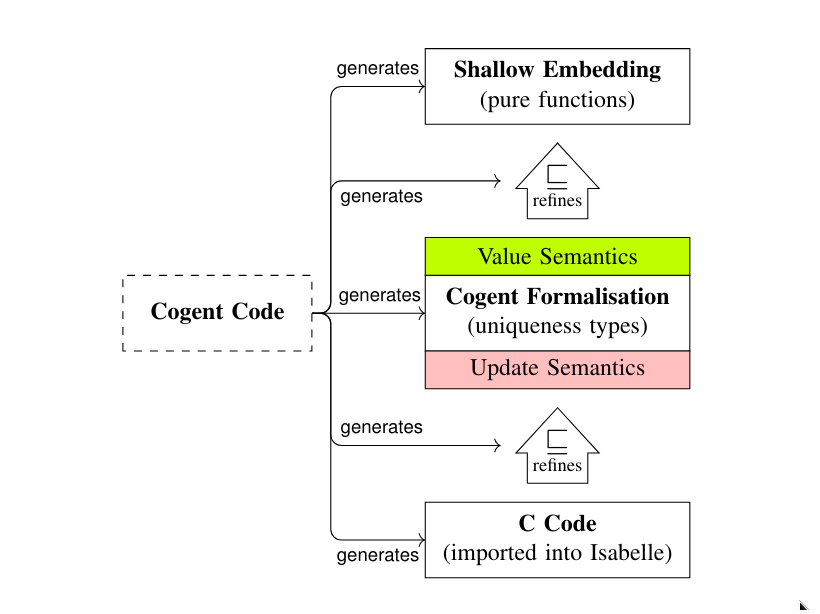
\includegraphics[width=0.85\textwidth]{figures/dargent_pipeline.png}
    \caption{The Cogent refinement framework (adapted from \cite{dargent_isola}). 
  Each box represents an embedding of the same Cogent program within Isabelle/HOL, 
  and arrows denote refinement proofs that establish semantic equivalence between 
  successive representations. 
  This verified foundation underpins later extensions such as Dargent, 
  which introduces declarative data-layout descriptions within the Cogent toolchain.}
    \label{fig:dargent_pipeline}
\end{figure}

\subsubsection{Extending the Lineage}
Earlier foundational work by \textbf{Tuch} (2008) formalized C's
pointer and heap semantics and Isabelle, laying the groundwork for verified
reasoning about memory at the byte level~\autocite{tuch2008formal}. More
recently, efforts such as a \textbf{Cornucopia} for CHERI
architectures~\autocite{filardo2020cornucopia} continue to
push forward verified compilation toward more realistic representations of
machine memory. 

Cedar builds directly on this insight. It seeks to extend the
extend the idea of \textbf{type-layout separation} and layout well-formedness
checking to the broader C ecosystem, without imposing
Cogent's functional restriction or proof obligations. In this sense, Cedar
generalized the principles pioneered by Dargent, bringing declarative layout
specifications to conventional systems programming. 

\subsection{Declarative and Domain-Specific Layout Languages}
While verified compilers focus on proving that compilers focus on
proving that compilation preserves meaning, a complementary tradition in
language design makes the data \textit{representation} explicit
through \textbf{declarative schema or layout languages}. These languages
allow programmers to describe binary formats at a high level, from which
parsers, serializers, and accessors, can be generated automatically.
Their goal is not proof of semantic equivalence, but \textbf{automation,
maintainability, and safety} in specifying
how structured data maps to bytes.

\subsubsection{Academic Layout Description Languages}
Early research systems such \textbf{PADS} and \textbf{DataScript} pioneered
declarative specifications of binary
data~\autocite{fisher2005pads,back2002datascript}. PADS introduced a system for
ad-hoc data formats, enabling automatic parser generation and providing
basic static checks such as field coverage
and alignment consistency. 
\textbf{DataScript}~\autocite{back2002datascript}, developed at Stanford,
treated binary layouts as first-class constructs: programmers defined bit-level
field structures and constraints, and the compiler generated Java classes to
read and write them. These languages were influential in showing that low-level
binary parsing could be expressed declaratively rather than through manual
bit-twiddling code. 

\subsubsection{Industrial Serialization Frameworks}
Many of these academic ideas re-emerged in modern industrial
frameworks designed for cross-platform serialization and
inter-process communication. Tools such as
\textbf{FlatBuffers}~\autocite{flat_buffers} and 
\textbf{Cap'n Proto}~\autocite{capn_proto_serialization}
use \textbf{interface definition languages} (IDLs) to describe data
schemas from which efficient, type-safe code is generated automatically.
These frameworks guarantee binary compatibility across architectures
and languages, reducing the likelihood of layout mismatches between
communicating components.

The \textbf{Cap'n Proto} and \textbf{FlatBuffers} tools focus on
zero-copy access: data can be read directly from the
serialized buffer without immediate unmarshalling. This design
aligns with the performance goals of systems programming but
constrains data access to API-generated methods
rather than arbitrary pointer arithmetic. A recent survey by
\textbf{Vioti and Kinderkhedia (2022)}  catalogues these binary specifications
and highlights trade-offs between expressiveness, schema evolution, and
safety~\autocite{viotti2022survey}. 

Recent work has begun on examining these tools from a \textbf{security
pers}. \textbf{Lilly Sell's (2024)} analyses the schema semantics of
FlatBuffers and its implementation to identify classes of layout
vulnerabilities and unsafe pointer usage~\autocite{sellsecurity}. The
study emphasizes that, despite their strong type systems, industrial
IDLs provide no formal guarantees about in-memory safety or field alignment
once data is accessed through unsafe code. These findings
underline that even modern frameworks remain
vulnerable when low-level layout details escape the boundaries of their
generated APIs.

\subsubsection{Comparing Declarative Layout Languages}
Declarative layout frameworks share several design principles:
\begin{enumerate}
    \item they separata \textit{logical structure} from\
    \textit{physical representation},
    \item they generate accessors and parsers automatically; and
    \item they provide at least partial checks for field consisteny or
    alignment.
\end{enumerate}

However, they typically operate in \textbf{controlled environments}—either
within managed runtimes or through generated API layers—and are not designed
for \textbf{arbitrary pointer-level operations} common in systems code.
Their safety guarantees therefore stop at the interface boundary: once raw
memory is accessed directly, correctness again depends on the programmer.

%Table of compariosn of DSL (PADSm DataScript, BinX, FlatBuffers, Cap'n Proto
%Avro and Cedar)

Cedar builds on this lineage by re-introducing declarative layout control
\textit{within C} itself. It inherits Dargent's separation between logical
physical layouts but targets a more permissive,
imperative environment. Where existing DSLs stop at schema generation,
Cedar amis to provide static well-formedness checking and direct compatibility
with verified C toolchains such as CompCert. In doing so, it connects the
two worlds of declarative layout description and
verified low-level systems programming. 

%FFigure of Declarative layout timeline
%PADS -> DataScript -> BINX -> Industrial IDLS -> Dargent -> Cedar

\subsection{Runtime Safety and Analysis Tools}
When low-level layout errors escape compile-time detection, developers rely on
\textbf{runtime instrumentation} and \textbf{static or dynamic analysis} to
locate faults.
These tools do not prevent misuse of memory, but they help identify common
classes of errors such as buffer overflows, uninitialized reads, and invalid
pointer dereferences.

\subsubsection{Dynamic Analysis Tools}
Dynmaic instrumentation frameworks such as
\textbf{Valgrind/Memcheck}~\autocite{valgrind} monitor every
memory access to detect invalid reads and writes at byte granularity.
Compiler-based sanitizers—including \textbf{AddressSanitizer (ASAN)},
\textbf{UndefinedBehaviorSanitizer (UBSAN)}, and
\textbf{MemorySanitizer (MSan)}—insert checks into generated code to catch
access errors and violations of the C standard at runtime~\autocite{ubsan,asan}.
These tools have been widely adopted in testing and continuous-integration
pipelines because they can reveal elusive bugs that arise from
undefined behavior, alignment faults,
and mis-computed offsets.

However, such techniques are inherently \textbf{reactive}. They only
detect errors along exercised execution paths and their effectiveness
depends heavily on the completeness of test coverage.
In addition, instrumentation typically incurs in non-trivial
runtime overhead—Valgrind can slow execution by an order of magnitude—making
these tools unsuitable for production or embedded environments. While
they are indispensable for debugging, they provide \textbf{no guarantee}
that untested code is free from layout mismatches or that binary
representations remain consistent across architectures. 

\subsubsection{Static Analysis and Type-Based Approaches}
Complementary static analyses attempt to infer
memory usage and pointer relationships directly from source code.
Tools such as \textbf{Cclyzer} perform
\textbf{points-to and structure-sensitive analysis} to detect potential
type violations~\autocite{balatsouras2016structure}. 
These methods can flag probable bugs before execution, but their
results depend on heuristics and may yield false positives or incomplete
coverage for low-level bit-manipulation code. Static analyses
are particularly challenged by C's weak type system and unrestricted
pointer arithmetic, which blur the boundary between logical structure
and physical representation.

\subsubsection{Safer Systems Languages}
Alongside external tools, modern systems languages incorporate
safety directly into their type systems. \textbf{Rust}, for
example, enforces memory safety through ownership and borrowing rules
that prevent data races and use-after-free errors at
compile time~\autocite{Rust_lang,Rust_systems}. Attributes
such as \texttt{\#\[repr(C)\]} allow Rust structures to
maintain binary compatibility with C while preserving the language
safety guarantees~\autocite{rust_repr}. However, Rust's model does not
eliminate layout variability entirely: padding and alignment remain 
platform-dependent, and many performance-critical routines still
resort to \texttt{unsafe} code when manipulating bit-fields or
packed data~\autocite{unsafe_rust}.

Emerging projects such as \textbf{Carbon} aim to modernize C++ while
improving safety and tooling~\autocite{carbon_cpp_safety}. Yet their
treatment of low-level representation is still evolving;
fine-grained layout control and verified layout correctness are not
current design goals.

These language-level solutions demonstrate the growing demand
for safer systems programming, but they also show
how difficult it is to combine \textbf{fine-grained control} with
\textbf{formal assurance}. Cedar occupies a complementary niche: it does
not replace C or enforce a new ownership mode, but instead
introduces \textbf{declarative layout specification} within existing
C codebases, addressing correctness at the representation layer. 

\subsubsection{Hardware-Assisted Memory Safety}
Recent research explores hardware extensions to enforce spatial and temporal
safety directly in the architecture. The \textbf{Capability Hardware
Enhanced RISC Instructions (CHERI)} architecture introduces
bounds and permissions to pointers, preventing many classes of buffer overflow
and use-after-free errors\autocite{filardo2020cornucopia}. Building on
this model, \textbf{Cornucopia} introduces efficient mechanisms for temporal
safety in CHERI heaps. Such approaches complement compiler instrumentation
by catching illegal accesses in hardware, greatly reducing overhead and enabling
fine-grained isolation between components.

Despite their effectiveness, these mechanisms do not reason about
\textbf{representation correctness}: they guarantee that accesses stay within
allocated bounds, not that the bytes being accessed correspond
to the intended logical structure. A program can be spatially safe
but still misinterpret a binary layout
if field offsets or bit-widths are wrong. Hardware capabilities thus solve
one aspect of memory safety—protecting allocation boundaries—while leaving
layout correctness to the programmer. 

\subsubsection{Positioning Cedar}
Runtime and static tools collectively enhance robustness but they remain
\textit{after-the-fact} defenses. They identify violations of memory
safety rather than enforcing \textit{design-time correctness} of layouts.
Cedar approaches the problem from the opposite direcion: by
\textbf{declaring layouts explicitly} and checking their compatibility
with corresponding C types before compilation, it aims
to prevent entire categories of representation errors that dynamic tools
can only detect later. Where Valgrind and sanitizers
ensure that a memory access is valid, Cedar, ensures that the 
access corresponds to the \textit{right bytes}. In this sense,
Cedar complements runtime verification and hardware enforcement, providing a
static foundation on which these broader safety mechanisms can rely.


\subsection{Summary and Research Gap}
This chapter has reviewed the landscape work related to data-layout
control and memory safety in systems programming. The discussion
began with the \textbf{C memory model}, where representation
details such as alignment, padding and field order remain
underspecified and vary across compilers and architectures.
These ambiguities complicate reasoning about correctness and performance in
context such as device drivers and protocol stacks. Subsequent
sections examined how \textbf{verified compilers} and \textbf{languages},
exemplified by CompCert, Cogent and Dargent, have provided rigorous guarantees
about program semantics and layout correctness—but only within constrained or
abstracted settings. Other efforts, from \textbf{declarative layout DSLs} like
PADS and DataScript, to \textbf{industrial frameworks} such as FFlatBuffers
or Cap'n Proto, have demonstrated that high-level schema descriptions
can improve maintainability and portability, albeit without
formal assurance for in-place C data structures. Finally, the chapter
considered \textbf{runtime tools, hardware capabilities}, and \textbf{safer
systems languages} such as Rust, which mitigate many classes of memory errors
but do not address the root of the problem of explicitly specifying and
verifying layout semantics.

Across these approaches, a consistent limitation emerges. Verified compilers
assume layouts are correct but cannot check them. Declarative frameworks desribe
layouts but operate outside the C toolchain. Runtime tools detect violations
only after execution. None provide a \textbf{language-integrated, static
guarantee} that a C data structure's physical representation corresponds to its
intended logical form.

\textbf{Cedar} aims to bridge this gap. It brings declarative layout
philosphy of Dargent into the C ecosystem, allowing programmers to define
and check binary layouts directly alongside
their types. By separating logical structure from physical representation,
performing static well-formedness checks and generating cohesive C artifacts,
Cedar seeks to make low-level layout design both
expressive and reliable. The next chapter presents the
\textbf{design methodology} and \textbf{systems architecture} underpinning
this approach, outline how Cedar's compiler pipeline and language
features were developed and evaluated. 